\section{Simulation}

\subsection{Motivation für Simulationen}
\begin{itemize}
	\item Das Verhalten kann mittels Simulationen analysiert werden
	\item Mit Simulationen können Zeiten verkürzt werden
	\item Durch Simulationen kann die Reaktion der Steuerung auf Ausnahmesituationen überprüft werden
\end{itemize}

\subsection{Vernünftige Eingabewerte}
Ablauf einer Simulation: Einem Simulator werden vernünftige Eingabewerte gegeben und seine Reaktion darauf überprüft.
\subsubsection{Reale Eingabewerte für Simulatoren}
\begin{itemize}
	\item Reale, "'vernünftige"' Eingabewerte entsprechen möglichst gut der Realität
	\item Häufig sollen bei Simulationen zufällige Eingabewerte verwendet werden, die nicht notwendigerweise gleichverteilt sind. Häufig vorkommende Verteilungen sind:
	  \begin{itemize}
	    \item Gleichverteilung
		\item Normalverteilung (Gauss'sche Glockenkurve)
		\item Rayleigh-Verteilung
		\item Weibull-Verteilung
	  \end{itemize}
	\item Die Simulationen sollen reproduzierbar sein.
\end{itemize}

\subsection{Zufallszahlen-Generator (Random Number Generator, RNG)}
\subsubsection{Zufallszahlen}
\begin{itemize}
	\item Echt zufällige Zahlen können nur durch einen physikalischen Prozess erzeugt werden, z.B. durch Würfel oder Thermisches Rauschen.
	\item Eine deterministische Maschine wie der Computer kann keine echt zufälligen Zahlen generieren (ausser mit zusätzlicher Hardware $\rightarrow$ siehe TRNG).
	\item Ein Computer kann immerhin pseudozufällige Zahlen liefern.
\end{itemize}

\subsubsection{Hardware True RNG (TRNG)}
\begin{itemize}
    \item Clock = LOW: Transistoren leiten und zwingen Node A und B auf Vcc
    \item Clock = rising edge: Transistoren sperren
    \item Node A und B pendeln sich auf eine mittlere Spannung ein, bevor sie aufgrund von thermischem Rauschen zufällig auf 0 oder 1 fallen (jeweils invertiert)
\end{itemize}

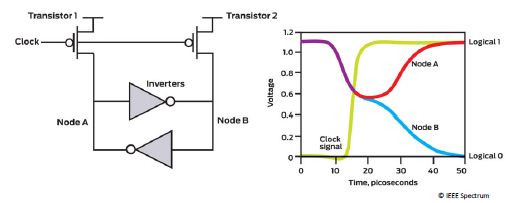
\includegraphics[width=0.7\textwidth]{images/Simulation/TRNG.png}

\subsection{Pseudozufallszahlen-Generator}
\subsubsection{Pseudozufällige Zahlen}
\begin{itemize}
	\item Pseudozufällige Zahlen sind deterministisch. Bei einem gegebenen Anfangswert (random seed) und gegebener Zufallszahlenfunktion ist die zufällige Zahlenfolge immer identisch. $\rightarrow$ hat den Vorteil, dass eine Simulation reproduzierbar wird.
	\item Der Nachteil ist, dass keine wirklich zufälligen Zahlen entstehen. Durch eine intelligent gewählte Funktion kann jedoch eine sehr hohe Periode der Folge erreicht werden, auch das Erraten der nächsten Zahl ist ohne Kenntnis des Random Seeds und der Funktion beinahe unmöglich.
\end{itemize}

\subsubsection{Forderungen}
\begin{itemize}
	\item Gleichverteilung
	\item Nächste Zahl nicht vorhersehbar
\end{itemize}

\subsubsection{Methoden}
\begin{itemize}
    \item Lineare Kongruenz: $r_{i+1} = (a \cdot r_i + c)\cdot mod (m)$
    \item Multiplikative Kongruenz (c=0): $r_{i+1} = (a \cdot r_i)\cdot mod (m)$
\end{itemize}

\subsubsection{rand() und srand()}
\begin{itemize}
    \item int rand(void); $\rightarrow$ liefert eine ganzzahlige Zufallszahl im Bereich von [0, RAND\_MAX] 
    \item void srand (unsigned int seed); $\rightarrow$ wird zur Initialisierung des Zufallszahlengenerators benutzt
\end{itemize}
Beispiel: 
\lstinputlisting[language=C++]{code/srand.cpp}

\subsubsection{Mapping von Zufallszahlen auf beliebige Bereiche}
rand() = Gleichverteilung\\

\begin{tabular}{|l|l|}
	\hline
	\textbf{rand()} & Liefert ganzzahlige Werte im Bereich [0, RAND\_MAX] \\ 
	\hline
	\textbf{rand() \% n} & Liefert Werte im Bereich [0, n-1] \\
	\hline
	\textbf{(double)rand()/RAND\_MAX} & Liefert Werte im Bereich [0, 1.0] \\ 
	\hline
	\textbf{(double)rand()/RAND\_MAX $\cdot$(b-a) + a} & Liefert Werte im Bereich [a, b] \\
	\hline
\end{tabular} \\\\

\textbf{Bei einer Umwandlung in eine ganze Zahl muss beachtet werden, ob runden oder abschneiden die richtige Operation ist.}\\

\subsubsection{Gleichverteilung von ganzen Zahlen in [low, high]}
\begin{lstlisting}
static_cast<int>(static_cast<double>(rand()) / (RAND_MAX + 1.0) * (high-low + 1)) + low
\end{lstlisting}
\begin{itemize}
  \item (RAND\_MAX + 1.0) ist notwendig, damit 0.0  $\leq$ u $<$ 1.0 (ohne 1.0) erzeugt wird. (RAND\_MAX + 1) gäbe einen int-Overflow
  \item (high – low + 1) ist notwendig, weil nach int konvertiert wird. Vor der int-Konversion gibt es dadurch bei [1,20] Zahlen im Bereich [0.0, 20.0[. Nach der Konversion werden nur die ganzzahligen Anteile verwendet.
  \item Das hinterste + low muss ausserhalb des Typecasts sein, andernfalls ergibt es eine Überhöhung bei 0, falls low $<$ 0 (alle Zahlen in ]-1.0, +1.0[ würden zu 0, d.h. doppelt so viele wie erlaubt)
\end{itemize}


\subsection{Wahrscheinlichkeitsverteilungen}
\subsubsection{Normalverteilung}
\begin{itemize}
    \item Kommt sehr häufig in der Praxis vor (Natur, Ingenieurwesen, Wirtschaft, etc.)
        \begin{itemize}
            \item Zufällige Messfehler um einen Sollwert
            \item Fertigungsschwankungen um einen Sollwert
        \end{itemize}
    \item Charakterisierung durch Mittelwert $\mu$ (häufigster Wert, Erwartungswert) und Standardabweichung $\sigma$  (Mass für Streuung, Breite der Glockenkurve)
    \item Eigenschaften der Normalverteilung:
        \begin{itemize}
            \item 68 \% aller Werte liegen innerhalb von $\mu \pm \sigma$
            \item 95 \% aller Werte liegen innerhalb von $\mu \pm 2\sigma$
            \item 99.7 \% aller Werte liegen innerhalb von $\mu \pm 3\sigma$
            \item 99.99 \% aller Werte liegen innerhalb von $\mu \pm 4\sigma$
        \end{itemize}
    \end{itemize}
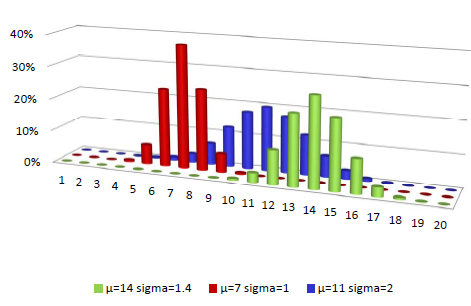
\includegraphics[width=0.5\textwidth]{images/Simulation/Normalverteilung.png}\\\\
\textbf{Zentraler Grenzwertsatz}\\
Die Summe von n unabhängigen, identisch verteilten Zufallszahlen stellt für n gegen unendlich eine Normalverteilung dar. \\\\ Eine Normalverteilung kann somit angenähert werden, wenn eine grosse Anzahl gleichverteilter Zahlen summiert wird. Die einfachste Methode ist die \textbf{Polarmethode von Marsaglia} (basiert auf Box-Muller-Algorithmus). Sie ergibt gute normalverteilte Zahlen und ist recht einfach zu berechnen (braucht "'nur"' einen Logarithmus und eine Wurzel).
\lstinputlisting[language=C++]{code/Polarmethode.cpp}

\subsubsection{Rayleigh Verteilung}
Eine Rayleigh-verteilte Zahl R kann aus zwei normalverteilten Zahlen $N_1$, $N_2$ mit Mittelwert 0 und Standardabweichung $\sigma$ wie folgt erhalten werden:\\
$R(\sigma) = \sqrt{N_1^2 + N_2^2}$\\
$R(\sigma) = \sigma \sqrt{-2 \ln(U)} \qquad U \neq 0$\\\\
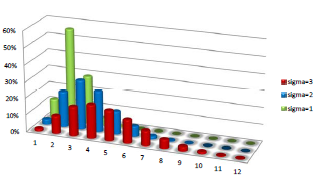
\includegraphics[width=0.5\textwidth]{images/Simulation/Rayleighverteilung.png}\\\\
Gemäss Formel braucht es für die Berechnung der Rayleigh-Verteilung zwei normalverteilte Zahlen.
\lstinputlisting[language=C++]{code/Rayleighmethode.cpp}

\subsubsection{Weibull Verteilung}
Die Dichtefunktion der Weibull-Verteilung kann mit 2 Parametern $\alpha$, $\beta$ wie folgt beschrieben werden:\\
$W_{\alpha,\beta}(x) = \alpha \cdot \beta \cdot x^\beta \cdot e^{-\alpha \cdot x^\beta}$ \\
\begin{wrapfigure}[3]{r}{0.51\textwidth}
    \vspace{-12pt}
    \centering
    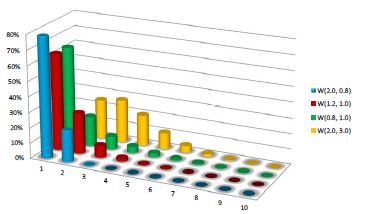
\includegraphics[width=0.50\textwidth]{images/Simulation/Weibullverteilung.png}
\end{wrapfigure}
\ 
\vspace{-5pt}
\begin{itemize}
	\item $\beta = 1$:  Exponentialverteilung
	\item $\beta = 3.4$:  Normalverteilung
	\item $\beta > 1$:  Alterndes System
\end{itemize} 
\ \\ \ \\ \ \\ \ \\ \ \\ \ \\
Eine Weibull-verteilte Zahl $W$ kann aus einer in $[0, 1.0[$ gleichverteilten Zahl $U$ mit folgender Formel berechnet werden:
\begin{equation}
	W(\alpha,\beta) = \beta \cdot (-\ln(1.0-U))^\frac{1}{\alpha}  \qquad U \neq 1.0
\end{equation}
\paragraph{Anwendung der Weibull-Verteilung}
\begin{itemize}
	\item Untersuchung von Lebensdauern in der Qualitätssicherung
	\item Materialermüdungen von spröden Werkstoffen
	\item Ausfälle von elektronischen Bauteilen
	\item Verteilung von Windgeschwindigkeiten (oft wird hierzu auch die Rayleigh-Verteilung herangezogen)
	\item Allgemein: Systeme mit im Laufe der Zeit steigender Ausfallrate (Systeme mit konstanter Ausfallrate sind exponentialverteilt)
\end{itemize}
